\documentclass[french, 12pt, aspectratio=2013]{beamer} 
% valeur possibles : article, proc, book, report, letter, slides
% options possibles : twosides (recto-verso), 12pt, 11pt, ... (taille de police), draft (brouillon)

% Language setting
% Replace `english' with e.g. `spanish' to change the document language
\usepackage[french]{babel}
\usepackage{amssymb}
\usepackage{shadowtext}

% Useful packages
\usepackage{amsmath}
\usepackage{graphicx}

%tableau pleine largeur
\usepackage{tabularx}

%faire des dessins
\usepackage{tikz}

\usepackage{algorithm}

\usepackage{color}
\newcommand{\com}[1]{\textcolor{olive}{#1}}
\usepackage[dvipsnames]{xcolor}
\definecolor{FFN}{HTML}{00AEFF}
\definecolor{MHA}{HTML}{FF9100}
\definecolor{Emb}{HTML}{F94C52}
\definecolor{Norm}{HTML}{AEC500}

\usepackage{listings}

\usepackage{appendixnumberbeamer}

% Theme choice:
\usetheme{Darmstadt}


\AtBeginSection[]{
    \begin{frame}{Sommaire}
        \tableofcontents[currentsection]
    \end{frame}
}


\title{Exploration de l'explicabilité de l'intelligence artificielle et application au traitement automatique de la langue naturelle}
\author{Marine DELVALLEZ}

\setbeamertemplate{footline}[frame number]
\setbeamertemplate{navigation symbols}{}

\begin{document}
\addtocounter{framenumber}{-1}
\begin{frame}[plain]
        
\includegraphics[scale=0.3]{images/Logo Minerve_RVB.jpg} \hfill
        
\includegraphics[scale=0.2]{images/France_2030_Logo_rouge_bleu_transparent.png} \hfill
        
\includegraphics[scale=0.3]{images/LIFO.png}
        \centering
        \Large Exploration de l'explicabilité de l'intelligence artificielle et application au traitement automatique de la langue naturelle\\
        \large Soutenance du Projet Immersion\\
        
        \vspace{2mm}
        \normalsize Marine DELVALLEZ \hfill
        \textit{Master 2 Informatique GPEx Minerve}\\
        \vspace{2mm}
        \centering \footnotesize 7 Janvier 2026 \\
    \end{frame}

\begin{frame}{Sommaire}
    \tableofcontents[]
\end{frame}

\section{Intelligence Artificielle et Modèles de Langue}
    \subsection{Définitions}
        \begin{frame}{Intelligence Artificielle}
            \begin{block}{Intelligence Artificielle}
                    \centering
                    \begin{tabular}{|c|c|}
                \hline
                    Comportement humain & Comportement rationnel \\
                    \hline
                    Raisonnement humain & Raisonnement rationnel\\
                    \hline
                \end{tabular}
            \end{block}
            \pause
            \emph{Données} : Images, Sons, Vidéo, Texte, Tables Attribut-Valeur, Entiers, Classes,...
            
            \pause
            \begin{block}{Tâche}
                Nature de donnée d'entrée + Nature de sortie + spécification
            \end{block} 
            \emph{Classification} : Texte $\to$ Classe, Condition\\
            \emph{Sous-titrage d'images} : Image $\to$ Texte, Décrire\\
            \emph{Traduction} : Texte $\to$ Texte, Changer la langue\\ 
            ...
        \end{frame}
        
        \begin{frame}{Grands Modèles de Langue}
        
            {\centering
            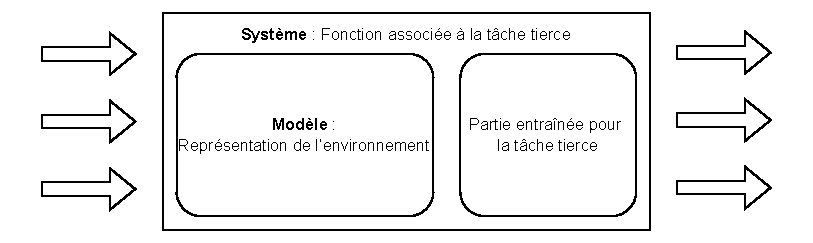
\includegraphics[width = \textwidth]{images/Modele-Systeme-Input-Output.drawio.pdf}}
        
            \emph{Exemple} : BERT pour la classification de texte
        \end{frame}
        
    \subsection{Le modèle Transformer}
        \begin{frame}{Architecture du Transformer \cite{vaswani_attention_2017}}
            \begin{columns}
                    \begin{column}{0.4\textwidth}
                        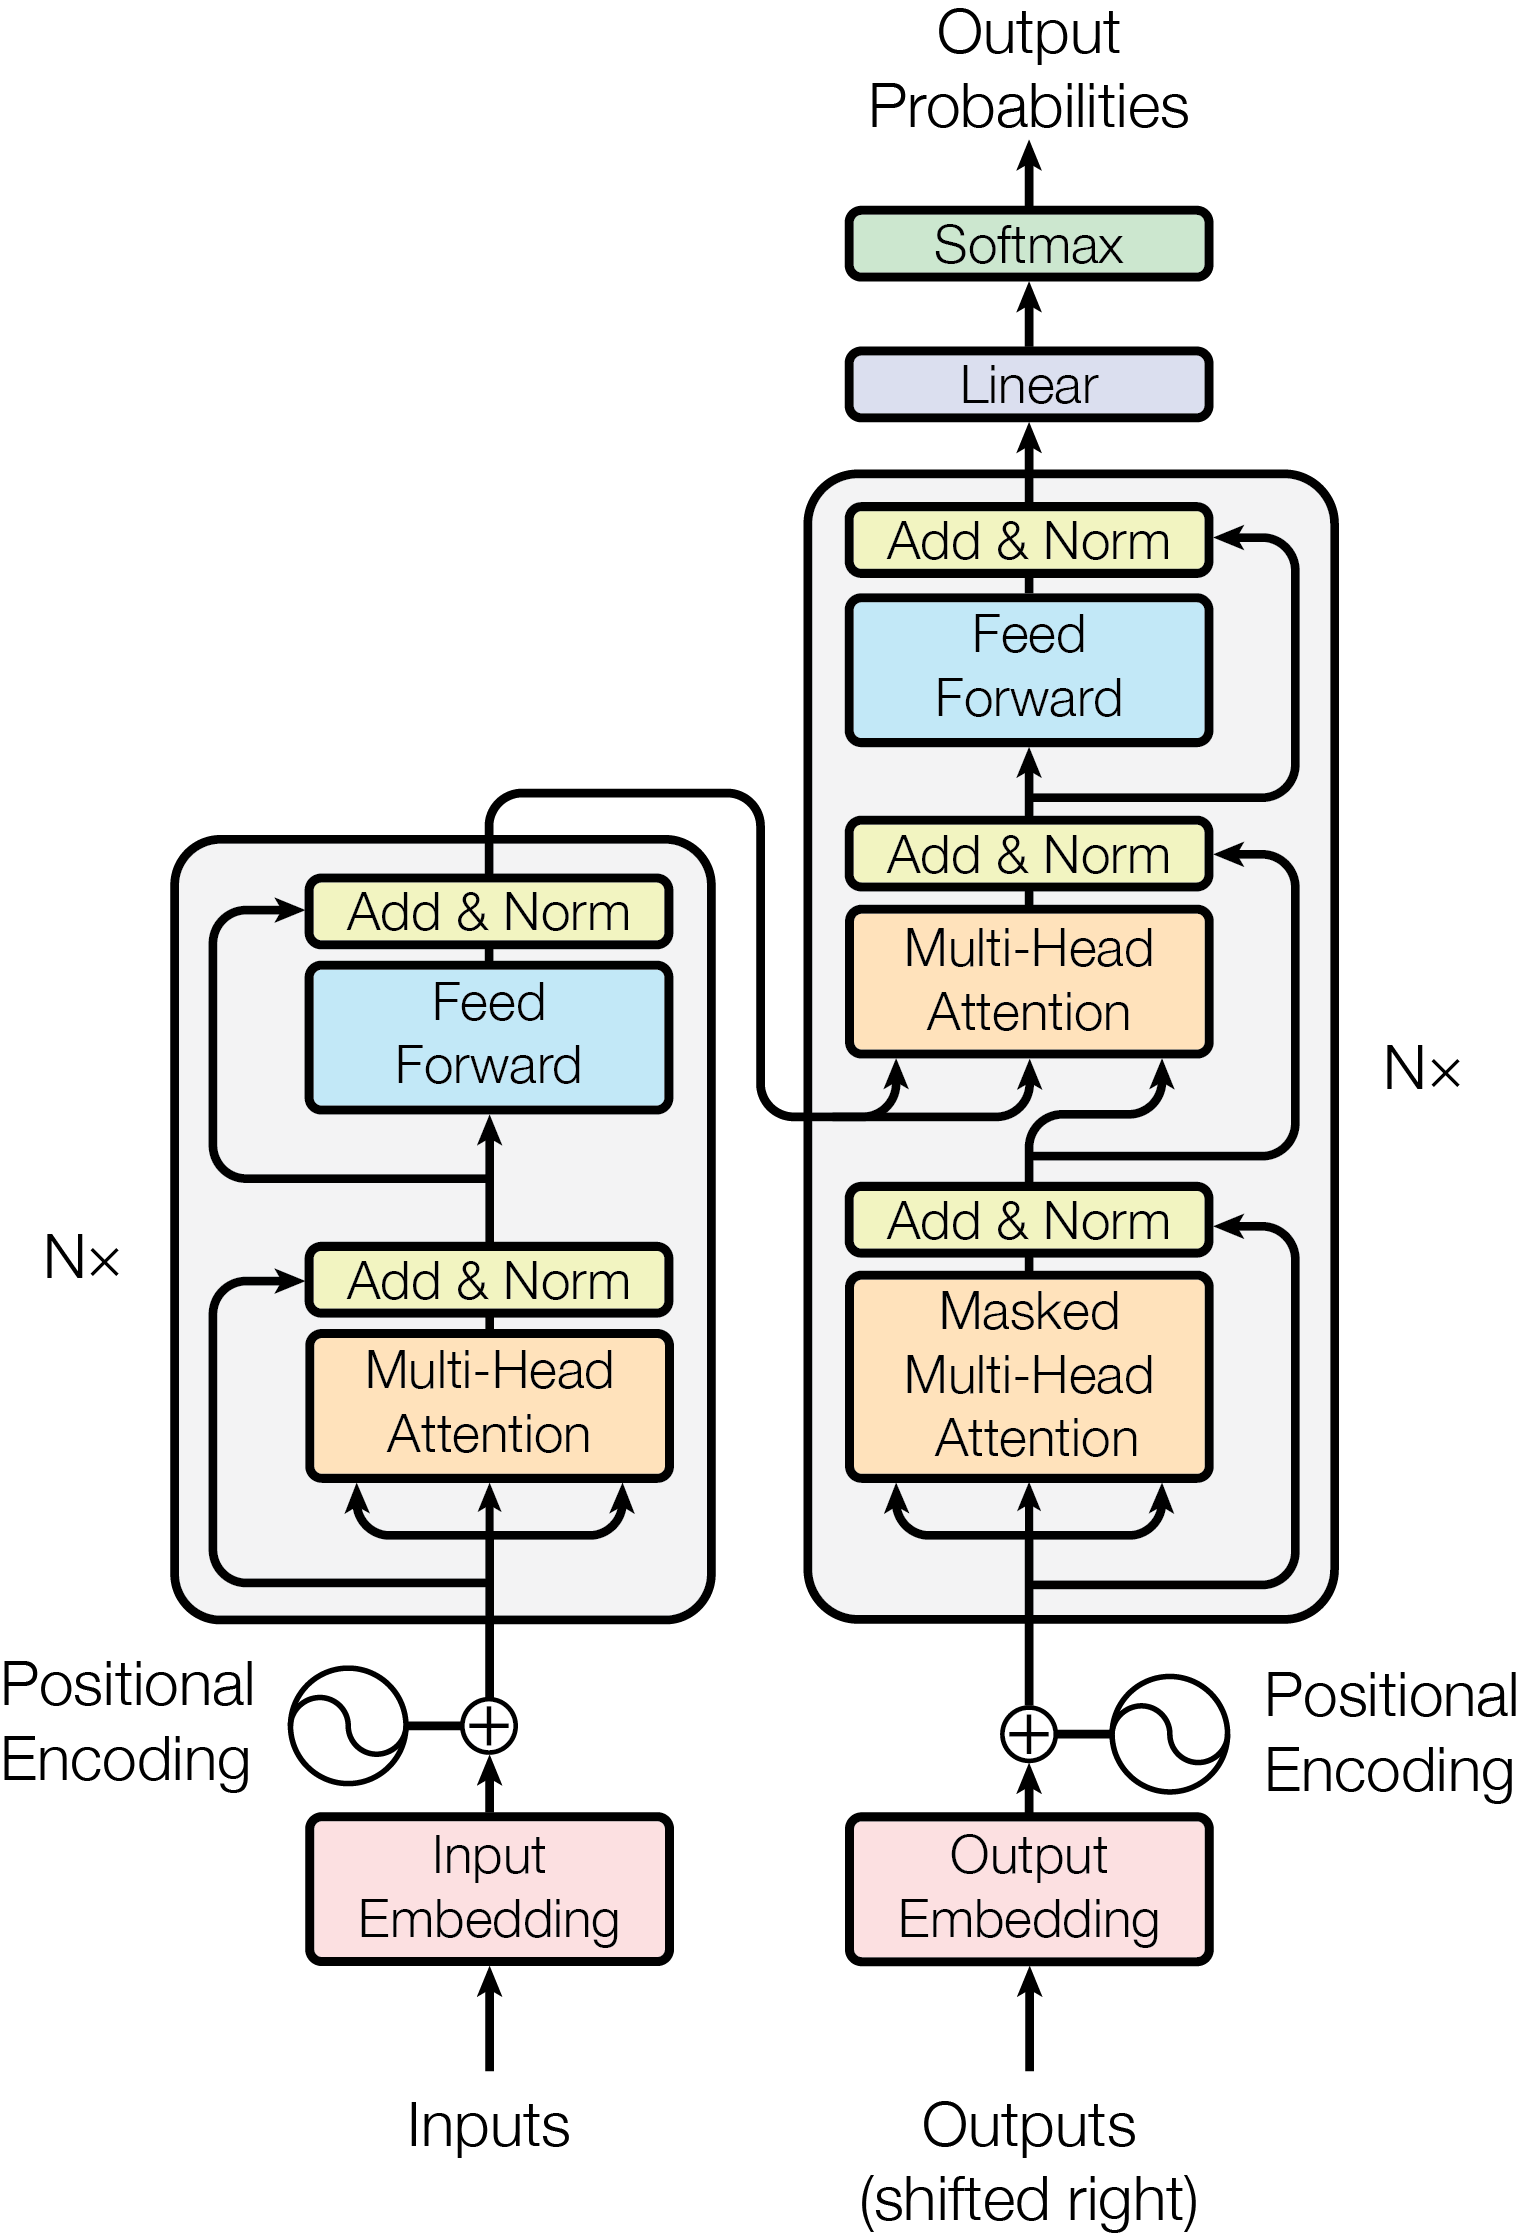
\includegraphics[height = 0.8\textheight]{images/Transformer_Vaswani-et-al2027.png}
                    \end{column}
                    \begin{column}{0.6\textwidth}
                        Composants Techniques:
                        \begin{itemize}
                            \item \textcolor{MHA}{Mécanisme d'attention multi-tête}
                            \item \textcolor{FFN}{Réseau de neurones}
                            \item Connexion résiduelle \&  %\shadowtext{
                            \textcolor{Norm}{Normalisation}%}
                            \item \textcolor{Emb}{Embedding} et Encoding positionnel
                        \end{itemize}
                        
                        \pause
                        Modèles dérivés du Transformer:
                        \begin{itemize}
                            \item BERT \cite{devlin_bert_2019}
                            \item GPT \cite{radford_improving_2018}
                            \item T5 \cite{raffel_exploring_2020}
                            \item $\dots$
                        \end{itemize}
                    \end{column}
            \end{columns}
                

        \end{frame}
        
        \begin{frame}{Mécanisme d'attention}
            \begin{columns}
                \begin{column}{0.5\textwidth}
                    \begin{figure}
                        \centering
                        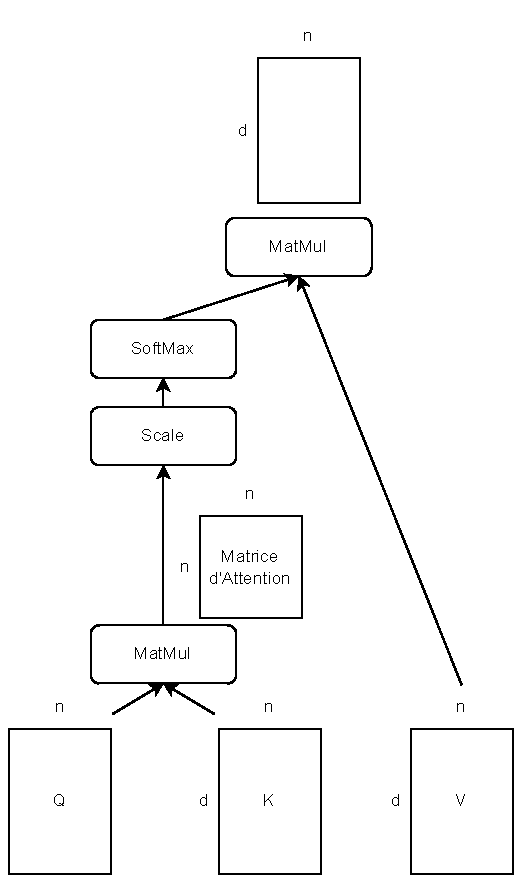
\includegraphics[height=0.65\textheight]{images/scaledDotProdAttention.drawio.pdf}
                        \caption{Scaled Dot Product Attention \cite{vaswani_attention_2017}}
                        \label{fig:scaledDotProductAttention}
                    \end{figure}
                \end{column}
                
                \begin{column}{0.5\textwidth}
                    \begin{figure}
                        \centering
                        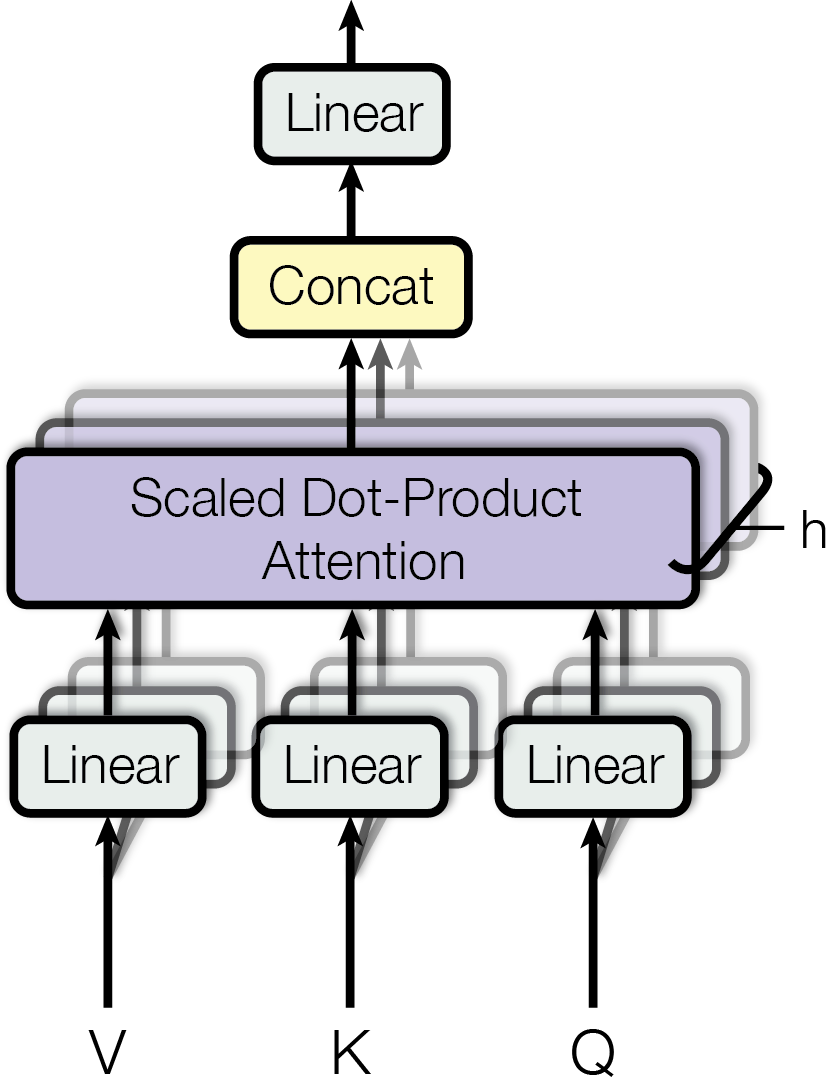
\includegraphics[width=0.6\textwidth]{images/MultiHeadAttention_Vaswani-et-al2017.png}
                        \caption{Mécanisme d'attention multi-tête \cite{vaswani_attention_2017}}
                        \label{fig:multi-headAttention}
                    \end{figure}
                \end{column}
            \end{columns}
        \end{frame}
        
        
    \subsection{Les modèles boite-noire}
        \begin{frame}{Modèle Boite-noire}
            \begin{block}{Modèle Boite noire}
                Modèles pour lesquels les processus de décision ne sont pas transparents pour l'humain
            \end{block}
            
            \emph{Problème} : Perte de confiance pour certains usages
        \end{frame}

\section{L'eXplicabilité de l'Intelligence Artificielle}

    \subsection{Définitions et enjeux}
        \begin{frame}{Définitions}
            %\com{
            %explicabilité de l'IA\\
            %explication}
            \begin{block}{Explicabilité de l'IA}
                Rendre \textbf<2>{humainement compréhensible} les raisons pour lesquelles un \textbf<3>{modèle effectue} une certaine prédiction \cite{garouani_investigating_2024, bell_its_2022}
            \end{block}
            \pause[4]
            \begin{block}{Comprendre}
                Être capable d'anticiper et/ou justifier le comportement du modèle \cite{bell_its_2022}
            \end{block}
            \pause[5]
            \begin{block}{Explication}
                Tout support rendant le processus de décision d'un modèle humainement intelligible.
            \end{block}
        \end{frame}
        
        
        \begin{frame}{Formes d'explication}
            \begin{columns}
                \begin{column}{0.5\textwidth}
                \centering
                    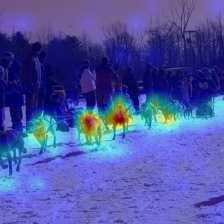
\includegraphics[width=0.7\textwidth]{images/37_grad_LRP.png}
                    \onslide<3->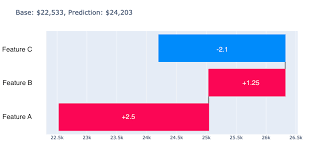
\includegraphics[width=\textwidth]{images/SHAP-Ill.png}  
                \end{column}
                \begin{column}{0.5\textwidth}
                    \onslide<2->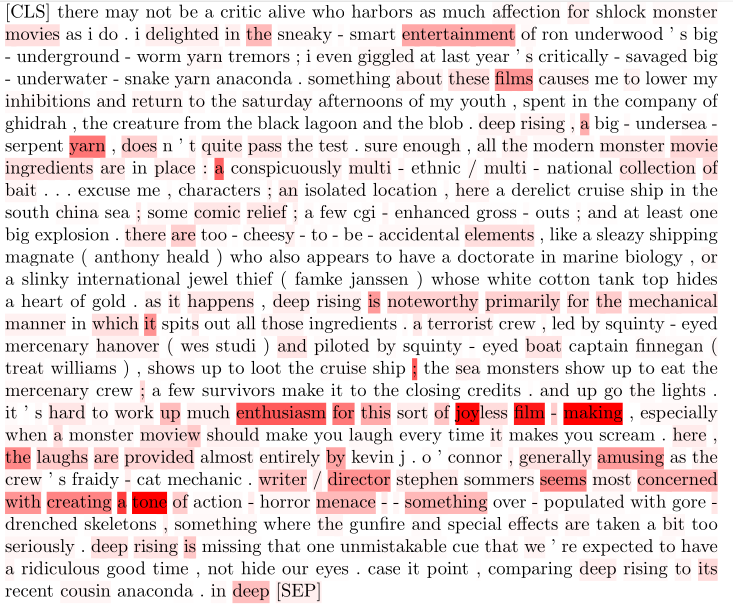
\includegraphics[width=\textwidth]{images/Their-CF.png}
                    \onslide<4->
                    \begin{align*}
                        C_1 &\iff A>B \wedge C \in \mathcal{S}\\
                        C_2 &\iff A<B \vee C \not\in \mathcal{S}
                    \end{align*}
                    
                \end{column}
            \end{columns}
            
        \end{frame}
        \begin{frame}{Temps de l'explicabilité}
        
            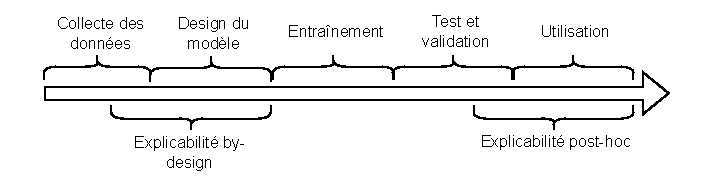
\includegraphics[width=\textwidth]{images/VieModele-TempsXAI.drawio.pdf}
            
            \vspace{5mm}
            \pause
            \begin{columns}
                    \begin{column}{0.5\textwidth}
                        Interprétabilité\\
                        \textit{Comment?}
                    \end{column}
                    \pause
                    \begin{column}{0.5\textwidth}
                        Explicabilité\\
                        \textit{Pourquoi?}
                    \end{column}
            \end{columns}
        \end{frame}
        
        
        \begin{frame}{Fidélité vs Accessibilité}
            \begin{block}{Des attendus contradictoires avec des conséquences}
                \begin{itemize}
                    \item sur-simplification $\implies$ confiance indue \cite{gilpin_explaining_2019}
                    \item sous-simplification $\implies$ inutilisable \cite{mersha_evaluating_2025} 
                \end{itemize}
            \end{block}
            \pause
            \begin{block}{Et un rapport avec le grand public compliqué}
                \begin{itemize}
                    \item Les explications créent une surcharge d'informations \cite{bell_its_2022}
                    \item Créé une crainte \cite{kastner_relation_2021}
                \end{itemize}
            \end{block}
        \end{frame}
    
    \subsection{Taxonomie des méthodes d'explication}
        \begin{frame}{Caractéristiques}
            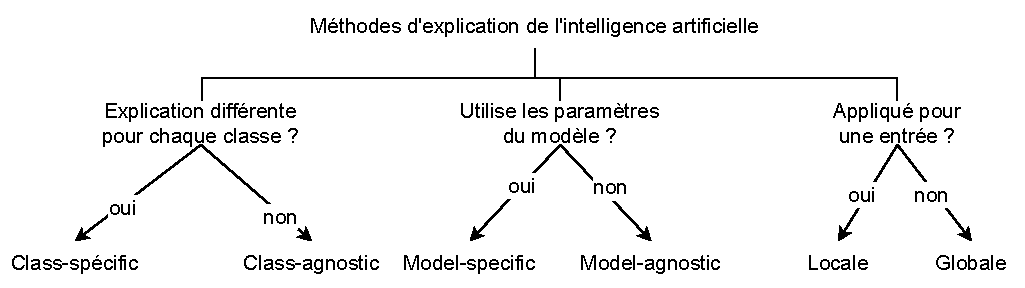
\includegraphics[width=\textwidth]{images/CaracteristiquesMethodeXAI.drawio.pdf}
        \end{frame}
        
        \begin{frame}{Stratégies}
            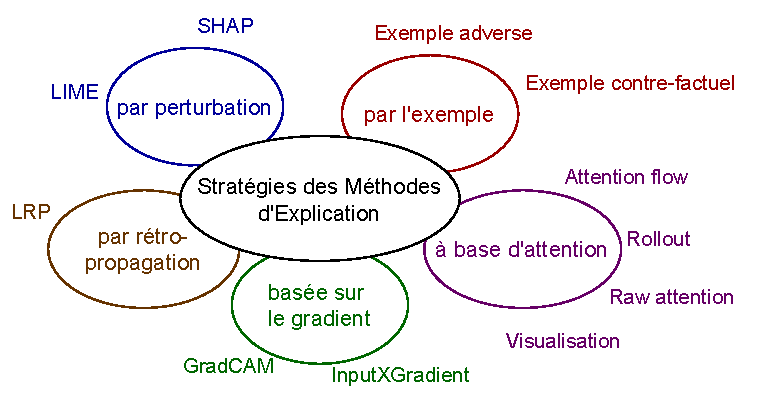
\includegraphics[width=\textwidth]{images/StrategiesMethodeXAI.drawio.pdf}
        \end{frame}
\iffalse        
        \begin{frame}{Méthode d'explication à base d'attention}
            \begin{block}{Matrice d'attention}
                Mesure l'importance de la relation entre chaque mot de l'entrée
            \end{block}

            \begin{columns}
                \begin{column}{0.5\textwidth}
                    \emph{Approches}:\\
                    \begin{itemize}
                        \item Visualisation
                        \item Exploitation directe d'une seule matrice 
                        \item Combinaison des matrices pour obtenir des scores
                    \end{itemize}
                \end{column}
                \begin{column}{0.5\textwidth}
                    \pause
                    \vspace{2mm}
                    
                    \emph{Remarques}: \\
                    \begin{itemize}
                        \item Exploitation d'une forme de représentation de l'entrée
                        \item mais prise en compte partielle du modèle
                        \item \cite{lopardo_attention_2024} remet en question cette approche d'un point de vue théorique
                    \end{itemize}
                \end{column}
            \end{columns}
            
        \end{frame}
        
        \begin{frame}{Méthode d'explication par propagation}
            \begin{block}{Intuition}
                Propager de la sortie vers l'entrée pour retrouver l'importance de chaque partie de l'entrée sur une sortie
            \end{block}
            \begin{figure}
                \centering
                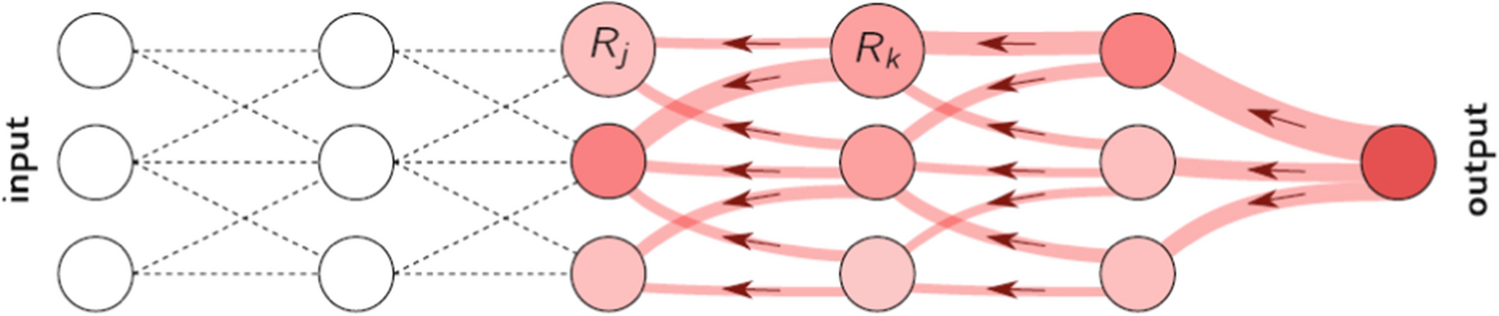
\includegraphics[width=\textwidth]{images/IllLRP.png}
                \caption{Intuition de Layer-wise Relevance Propagation \cite{bento_improving_2021}}
                \label{fig:IntuitionLRP}
            \end{figure}
            $
            R^{(n)}_j = \sum_i \frac{x_j^+ w_{ji}^+}{\sum_{j'} x_{j'}^+ w_{j'i}^+} R_i^{(n+1)}
            $
            où $v^+ = max(0,v)$
            \cite{montavon_layer-wise_2019}
        \end{frame}
        
        
        \begin{frame}{Méthode d'explication par perturbation}
        \begin{block}{Intuition}
            Observer le comportement du modèle au voisinage d'une entrée et  l'impact des variations sur la prédiction.
        \end{block}
        \emph{Local Interpretable Model-agnostic Explanation (LIME)} : Soient $M$ un modèle et $x$ une entrée
            \begin{enumerate}
                \item Construire un ensemble $\mathcal{X}$ de versions perturbées de $x$
                \item Entraîner un modèle interprétable $M'$ sur $\mathcal{X}\times M(\mathcal{X})$
                \item L'interprétation de $M'$ est une approximation de $M$ au voisinage de $x$
            \end{enumerate}
        \end{frame}
\fi    
\section{Évaluer les méthodes d'explications}

    \subsection{Les attendus}
        \begin{frame}{Les attendus}
            \begin{block}{Attendus d'une explication \cite{gilpin_explaining_2019}}
                \begin{itemize}
                    \item Fidèle au raisonnement du modèle
                    \item Intelligible pour le public visé
                \end{itemize}
            \end{block}
            
            \pause
            \begin{block}{Attendus d'une méthode d'explication \cite{mersha_evaluating_2025}}
                \begin{itemize}
                    \item Robustesse %: Des entrées similaires ont des explications similaires.
                    \item Consistance %: Les explications d'une même entrée pour deux modèles différents sont aussi différentes que les modèles.
                    \item Contrastivité %: Les explications distinguent les différentes prédictions possibles.
                \end{itemize}
            \end{block}

        \end{frame}
        
    \subsection{Les approches}
        \begin{frame}{Les approches}
            \begin{itemize}
                \item Comparer à des explications canoniques
                \item Comparer les méthodes d'explication entre elles
                \item Évaluer individuellement
                \item Analyser théoriquement
            \end{itemize}
        \end{frame}
        \begin{frame}{Comparer les explications à des explications canoniques}
        
            \begin{block}{Idée}
                \begin{enumerate}
                    \item Définir une explication attendue
                    \item Calculer la performance de la méthode d'explication
                \end{enumerate}
                %Définir une explication attendue pour chaque modèle et calculer la performance de la méthode d'explication
            \end{block}
            \begin{itemize}
                \item La \emph{Ground Truth humaine} n'est pas adaptée
                \item Construire une Ground Truth à partir du modèle utilisé ?
                \item Explication \textit{idéale} ? \cite{neely_song_2022}
            \end{itemize}
            
        \end{frame}
        
        \begin{frame}{Comparer les méthodes d'explications entre elles}
            \begin{block}{Idée}
                \begin{enumerate}
                    \item Prendre une méthode d'explication comme référence
                    \item Comparer ses explications avec celles de la méthode d'explication évaluée
                \end{enumerate}
            \end{block}
            \begin{itemize}
                \item \emph{Approches différentes} d'une méthode à l'autre
                \item Suppose la méthode de référence \emph{idéale}
                \item Quel sens? \cite{neely_song_2022}
            \end{itemize}
        \end{frame}
        
        \begin{frame}{Évaluer individuellement}
                \begin{block}{Idée}
                    Utiliser des métriques indépendantes qui évaluent les attendus
                \end{block}
                \begin{itemize}
                    \item Définir les attendus (exhausivité)
                    \item Trouver des métriques qui correspondent
                    \item Besoin de métriques \emph{universelles} ou \emph{comparables}
                \end{itemize}
        \end{frame}
        
        \begin{frame}{Aparté : Cas du jugement humain}
        %\com{
        %qualitatif\\
        %biasié vers accessibilité\\
        %cout de réalistaion\\
        %personens différentes d'une évaluatoin à l'autre : comparabilité?}
        \begin{block}{Idée }
            Demander à des personnes d'évaluer la méthode à l'aide de critères définis
        \end{block}
        Mais
        \begin{itemize}
            \item Évaluation qualitative
            \item Risque de biais \cite{gilpin_explaining_2019}
            \item Difficile à réaliser 
            \item Problèmes de comparabilité 
        \end{itemize}
    \end{frame}
    
    \begin{frame}{Analyse théorique des méthodes d'explication}
        \begin{block}{Idée}
            \begin{enumerate}
                \item Reprendre les définitions mathématiques du modèle et de la méthode d'explication
                \item Juger les attendus d'un point de vue théorique
            \end{enumerate}
        \end{block}
        \begin{itemize}
            \item Modèles boite-noire
            \item Définir mathématiquement les attendus
            \item \textit{Ex : \cite{lopardo_attention_2024}}
        \end{itemize}
    \end{frame}
    
    \subsection{Retour sur les enjeux de l'évaluation des méthodes d'explication}
        \begin{frame}{Existence des idéaux}
            \begin{itemize}
                \item Explication \emph{idéale}
                \item Méthode d'explication idéale
                \begin{itemize}
                    \item Pas de consensus \cite{garouani_investigating_2024}
                    \item Une méthode \emph{universelle} est-elle possible? (ex: \cite{mersha_evaluating_2025})
                \end{itemize}
            \end{itemize}
        \end{frame}
        
        \begin{frame}{Comparaison}
            \begin{itemize}
                \item Les explications sont-elles comparables? \item Les méthodes d'explication sont-elles comparables?
                \item Les métriques donnent-elles des résultats comparables?
                \item Quel sens?
            \end{itemize}
        \end{frame}
        
        \begin{frame}{Universalité}
            \begin{itemize}
                \item Les méthodes d'explication sont-elles adaptées ...
                \begin{itemize}
                    \item ... à tous les modèles?
                    \item ... à toutes les tâches?
                \end{itemize}
                \item Les métriques sont elles adaptées à tous les méthodes d'explication?
            \end{itemize}
        \end{frame}

\section{Conclusion}

%\begin{frame}{Autres sujets abordés dans ce stage}
%    \com{peut-être à placer ailleurs/ prévoir une annexe}
%    \begin{itemize}
%        \item Autres méthodes d'explication
%        \item Explicabilité by-design
%        \begin{itemize}
%            \item Modèles neuro-symboliques
%            \item Modèles à base de concepts
%        \end{itemize}
%    \end{itemize}
%\end{frame}

\begin{frame}{Perspectives}
    \begin{itemize}
        \item Faire un bilan des attendus et des métriques existantes
        \item Comparer les méthodes d'explications en fonction de la tâche traitée par le système
        \begin{itemize}
            \item Déterminer des besoins spécifiques aux tâches impliquant du texte
            \item Évaluer la pertinence d'une métrique \emph{universelle}
        \end{itemize}
    \end{itemize}
\end{frame}

\bibliographystyle{apalike} %alpha
\bibliography{sample.bib}

\appendix
\section{Annexes}

\subsection{Architecture de BERT}
\begin{frame}{Architecture de BERT}
    \begin{figure}
        \centering
        \begin{minipage}[c]{0.33\textwidth}
            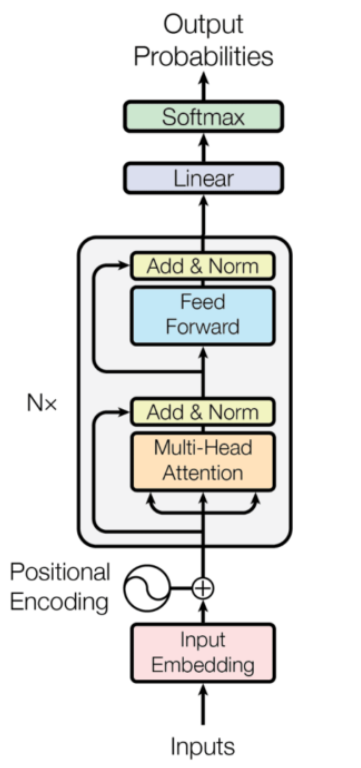
\includegraphics[height=0.85\textheight]{images/BERTArchi.png}
        \end{minipage}\hfill
        \begin{minipage}[c]{0.67\textwidth}
            \caption{Architecture du modèle BERT}
            \label{fig:BERT}
        \end{minipage}
    \end{figure}
\end{frame}
\subsection{Architecture de GPT}
\begin{frame}{Architecture de GPT}
    \begin{figure}
        \centering
        \begin{minipage}[c]{0.33\textwidth}
            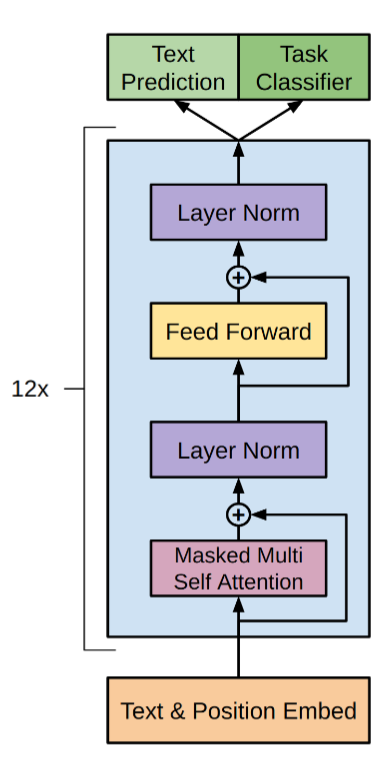
\includegraphics[height=0.85\textheight]{images/GPT_Radford-et-al2018.png}
        \end{minipage}\hfill
        \begin{minipage}[c]{0.67\textwidth}
            \caption{Architecture du modèle GPT \cite{radford_improving_2018}}
            \label{fig:GPT}
        \end{minipage}
    \end{figure}
\end{frame}
\subsection{Architecture de T5}
\begin{frame}{Architecture de T5}
    \begin{columns}
        \begin{column}{0.4\textwidth}
            \begin{figure}
                \centering
                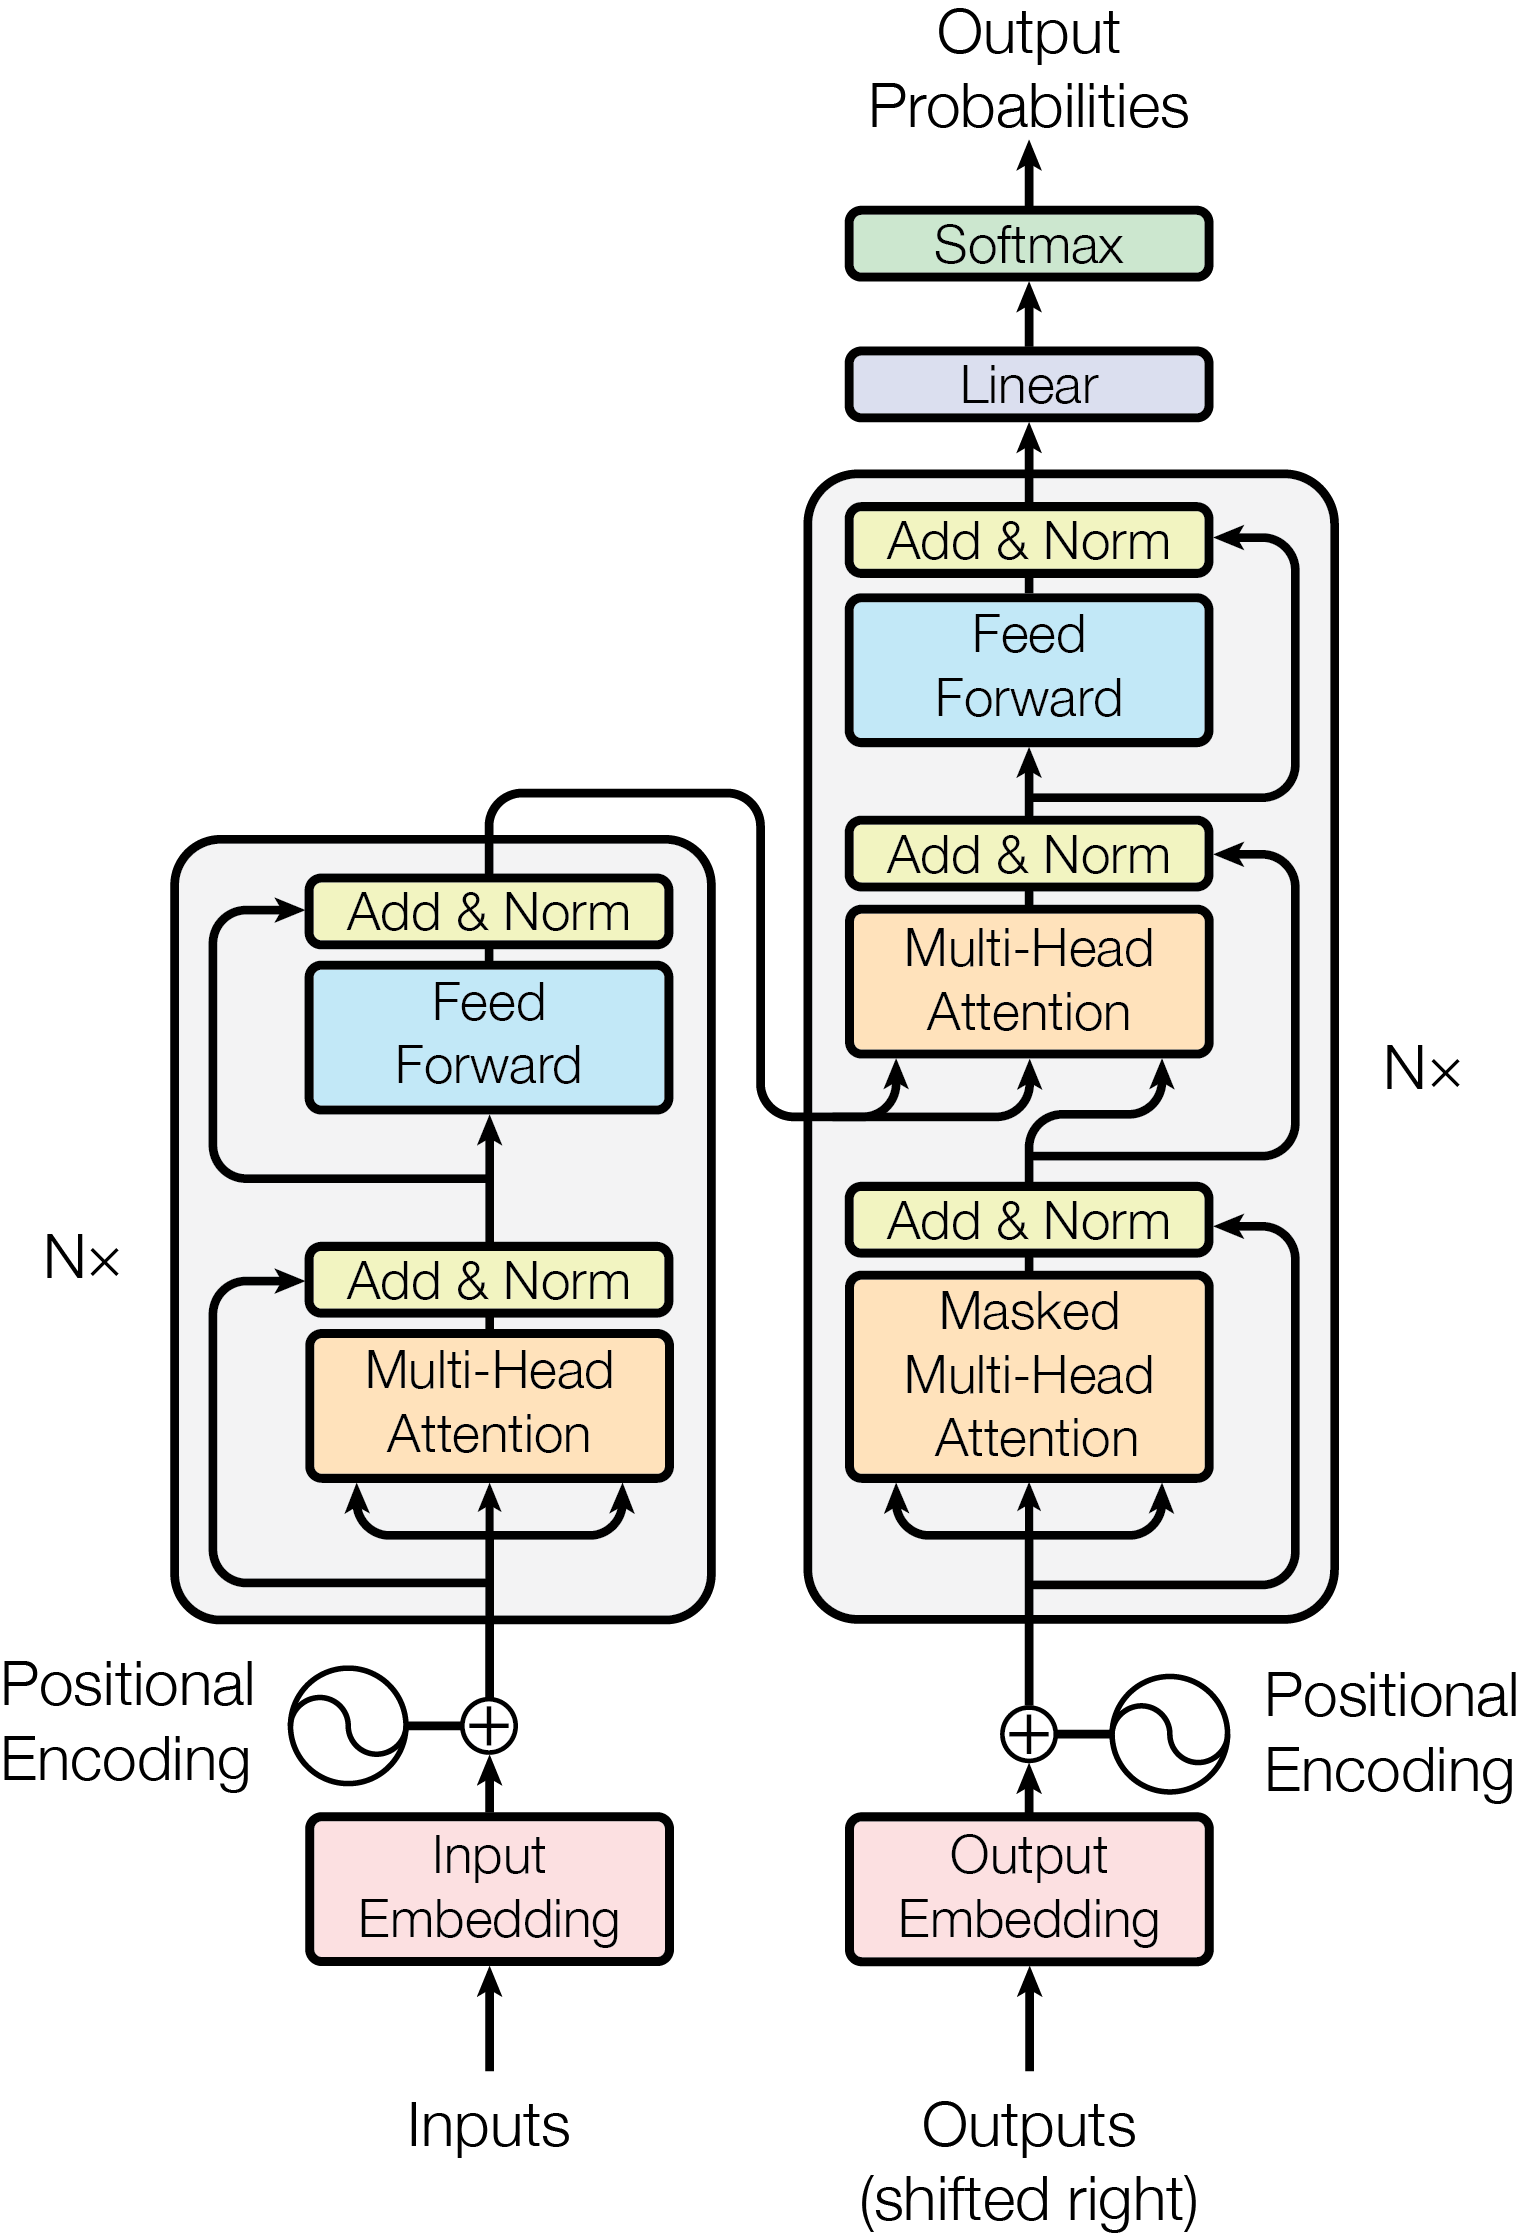
\includegraphics[width=0.75\textwidth]{images/Transformer_Vaswani-et-al2027.png}
                \caption{Architecture du Transformer \parbox{5em}{\cite{vaswani_attention_2017}}}
                \label{fig:Transformer}
            \end{figure}
        \end{column}
        \begin{column}{0.6\textwidth}
            Différences:
            \begin{itemize}
                \item Normalisation sans biais
                \item Connexion résiduelle après la normalisation
                \item Encodding positionnel relatif
            \end{itemize}
        \end{column}
    \end{columns}
\end{frame}

\subsection{Méthode d'explication à base d'attention}
\begin{frame}{Méthode d'explication à base d'attention}
    \begin{block}{Matrice d'attention}
        Mesure l'importance de la relation entre chaque mot de l'entrée
    \end{block}

    \begin{columns}
        \begin{column}{0.5\textwidth}
            \emph{Approches}:\\
            \begin{itemize}
                \item Visualisation
                \item Exploitation directe d'une seule matrice 
                \item Combinaison des matrices pour obtenir des scores
            \end{itemize}
        \end{column}
        \begin{column}{0.5\textwidth}
            \pause
            \vspace{2mm}
            
            \emph{Remarques}: \\
            \begin{itemize}
                \item Exploitation d'une forme de représentation de l'entrée
                \item mais prise en compte partielle du modèle
                \item \cite{lopardo_attention_2024} remet en question cette approche d'un point de vue théorique
            \end{itemize}
        \end{column}
    \end{columns}
    
\end{frame}

\subsection{Visualisation de l'attention}
\begin{frame}{Visualisation de l'attention}
\begin{figure}
    \centering
    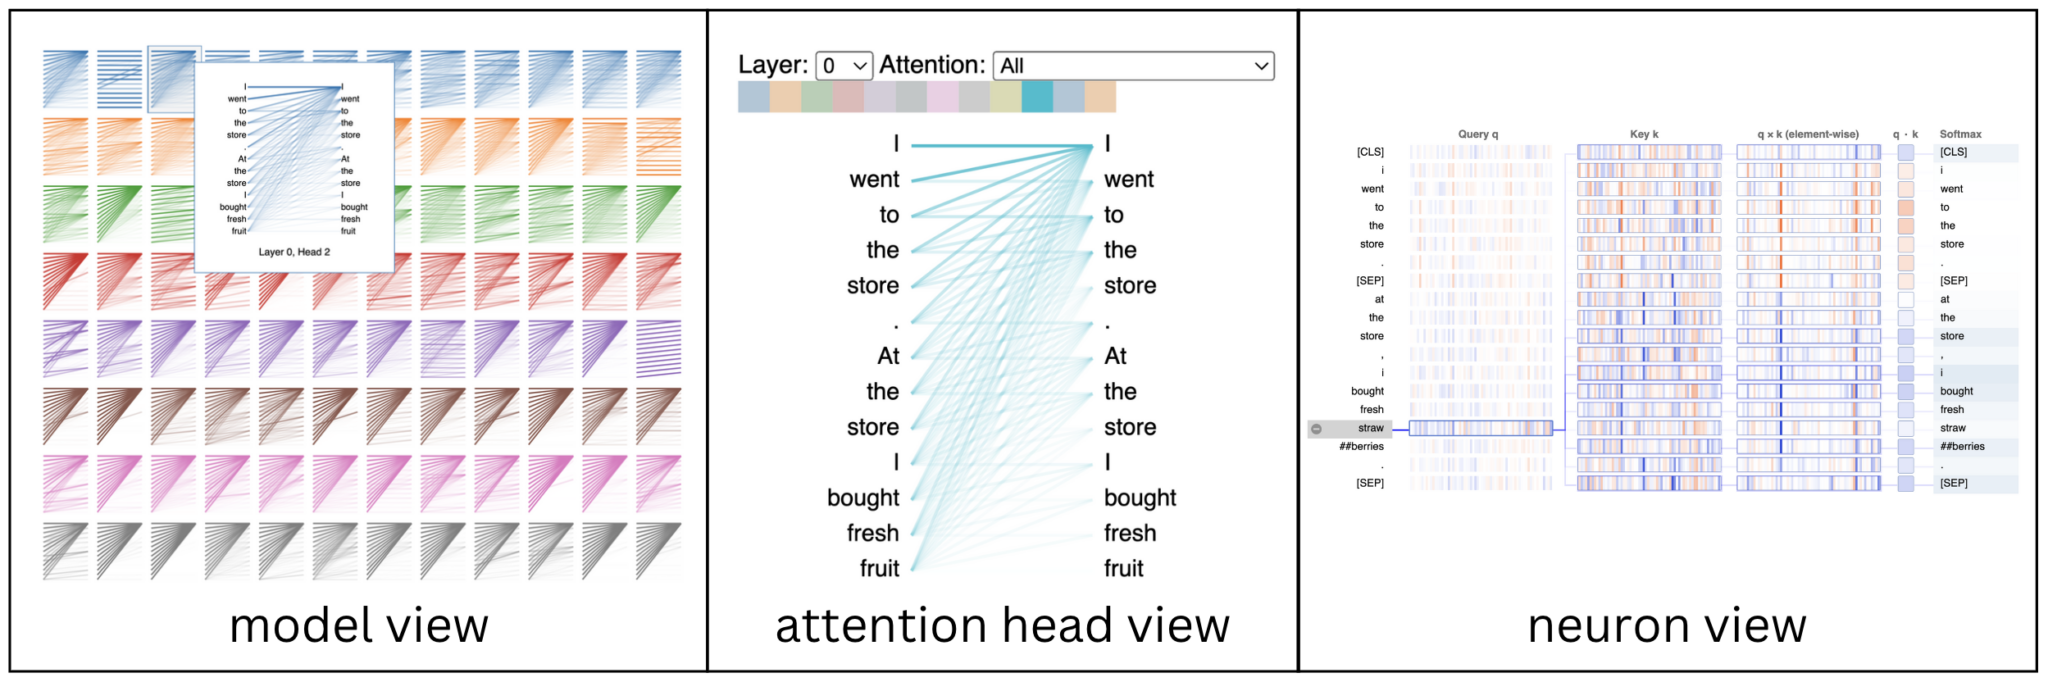
\includegraphics[width=\textwidth]{images/BertViz_allscales.png}
    \caption{BertViz \cite{vig_multiscale_2019} permet de visualiser le mécanisme d'attention à différentes échelles}
    \label{fig:bertviz}
\end{figure}
\end{frame}
   
\subsection{Méthode d'explication par propagation}     
\begin{frame}{Méthode d'explication par propagation}
    \begin{block}{Intuition}
        Propager de la sortie vers l'entrée pour retrouver l'importance de chaque partie de l'entrée sur une sortie
    \end{block}
    \begin{figure}
        \centering
        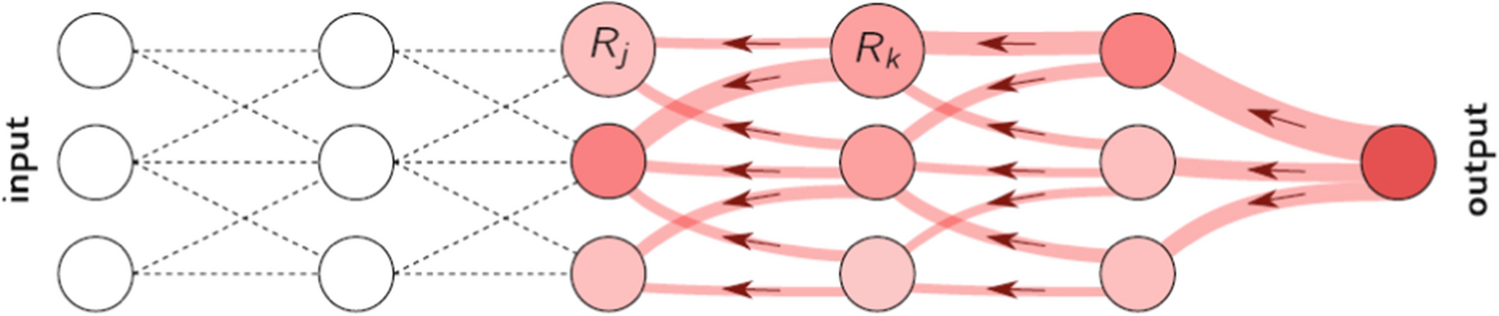
\includegraphics[width=0.9\textwidth]{images/IllLRP.png}
        \caption{Intuition de Layer-wise Relevance Propagation \parbox{5em}{\cite{bento_improving_2021}}}
        \label{fig:IntuitionLRP}
    \end{figure}
    $
    R^{(n)}_j = \sum_i \frac{x_j^+ w_{ji}^+}{\sum_{j'} x_{j'}^+ w_{j'i}^+} R_i^{(n+1)}
    $
    où $v^+ = max(0,v)$
    \parbox{5em}{\cite{montavon_layer-wise_2019}}
\end{frame}
        
\subsection{Méthode d'explication par perturbation}   
\begin{frame}{Méthode d'explication par perturbation}
    \begin{block}{Intuition}
        Observer le comportement du modèle au voisinage d'une entrée et  l'impact des variations sur la prédiction.
    \end{block}
    \emph{Local Interpretable Model-agnostic Explanation (LIME)} : Soient $M$ un modèle et $x$ une entrée
    \begin{enumerate}
        \item Construire un ensemble $\mathcal{X}$ de versions perturbées de $x$
        \item Entraîner un modèle interprétable $M'$ sur $\mathcal{X}\times M(\mathcal{X})$
        \item L'interprétation de $M'$ est une approximation de $M$ au voisinage de $x$
    \end{enumerate}
\end{frame}

\subsection{Méthodes d'explication par l'exemple}
\begin{frame}{Méthodes d'explication par l'exemple}
    \begin{center}
        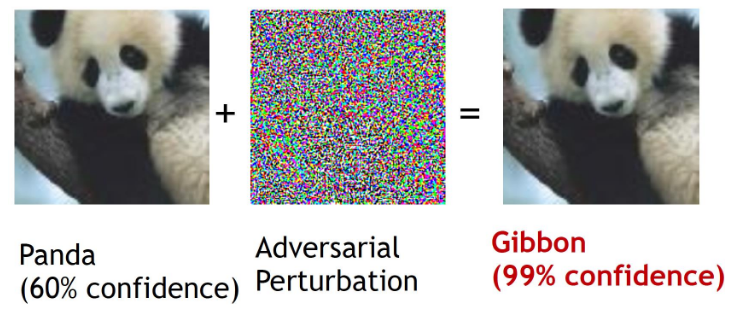
\includegraphics[width=0.6\textwidth]{images/AdversarialPerturbation_Panda.png}
        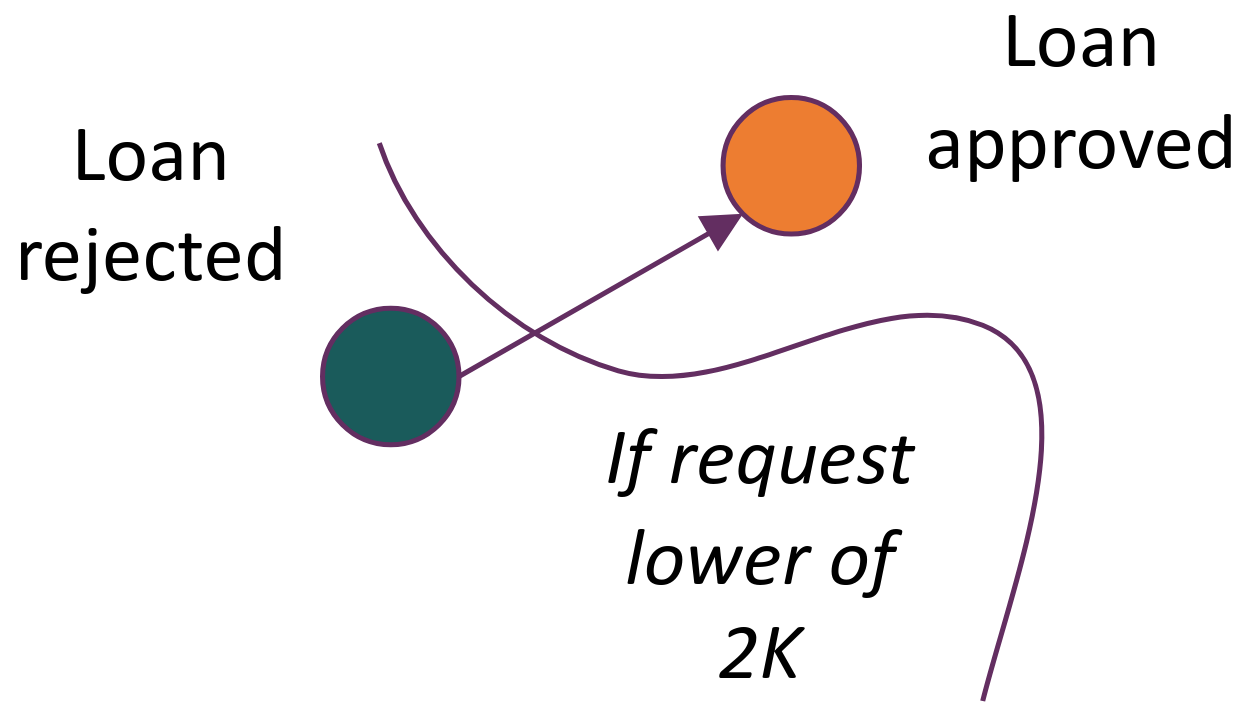
\includegraphics[width=0.4\textwidth]{images/ConterfactualExample.png}
    \end{center}
    
\end{frame}

\subsection{Modèles à base de concepts}
\begin{frame}{Modèles à base de concepts}
    \begin{figure}
        \centering
        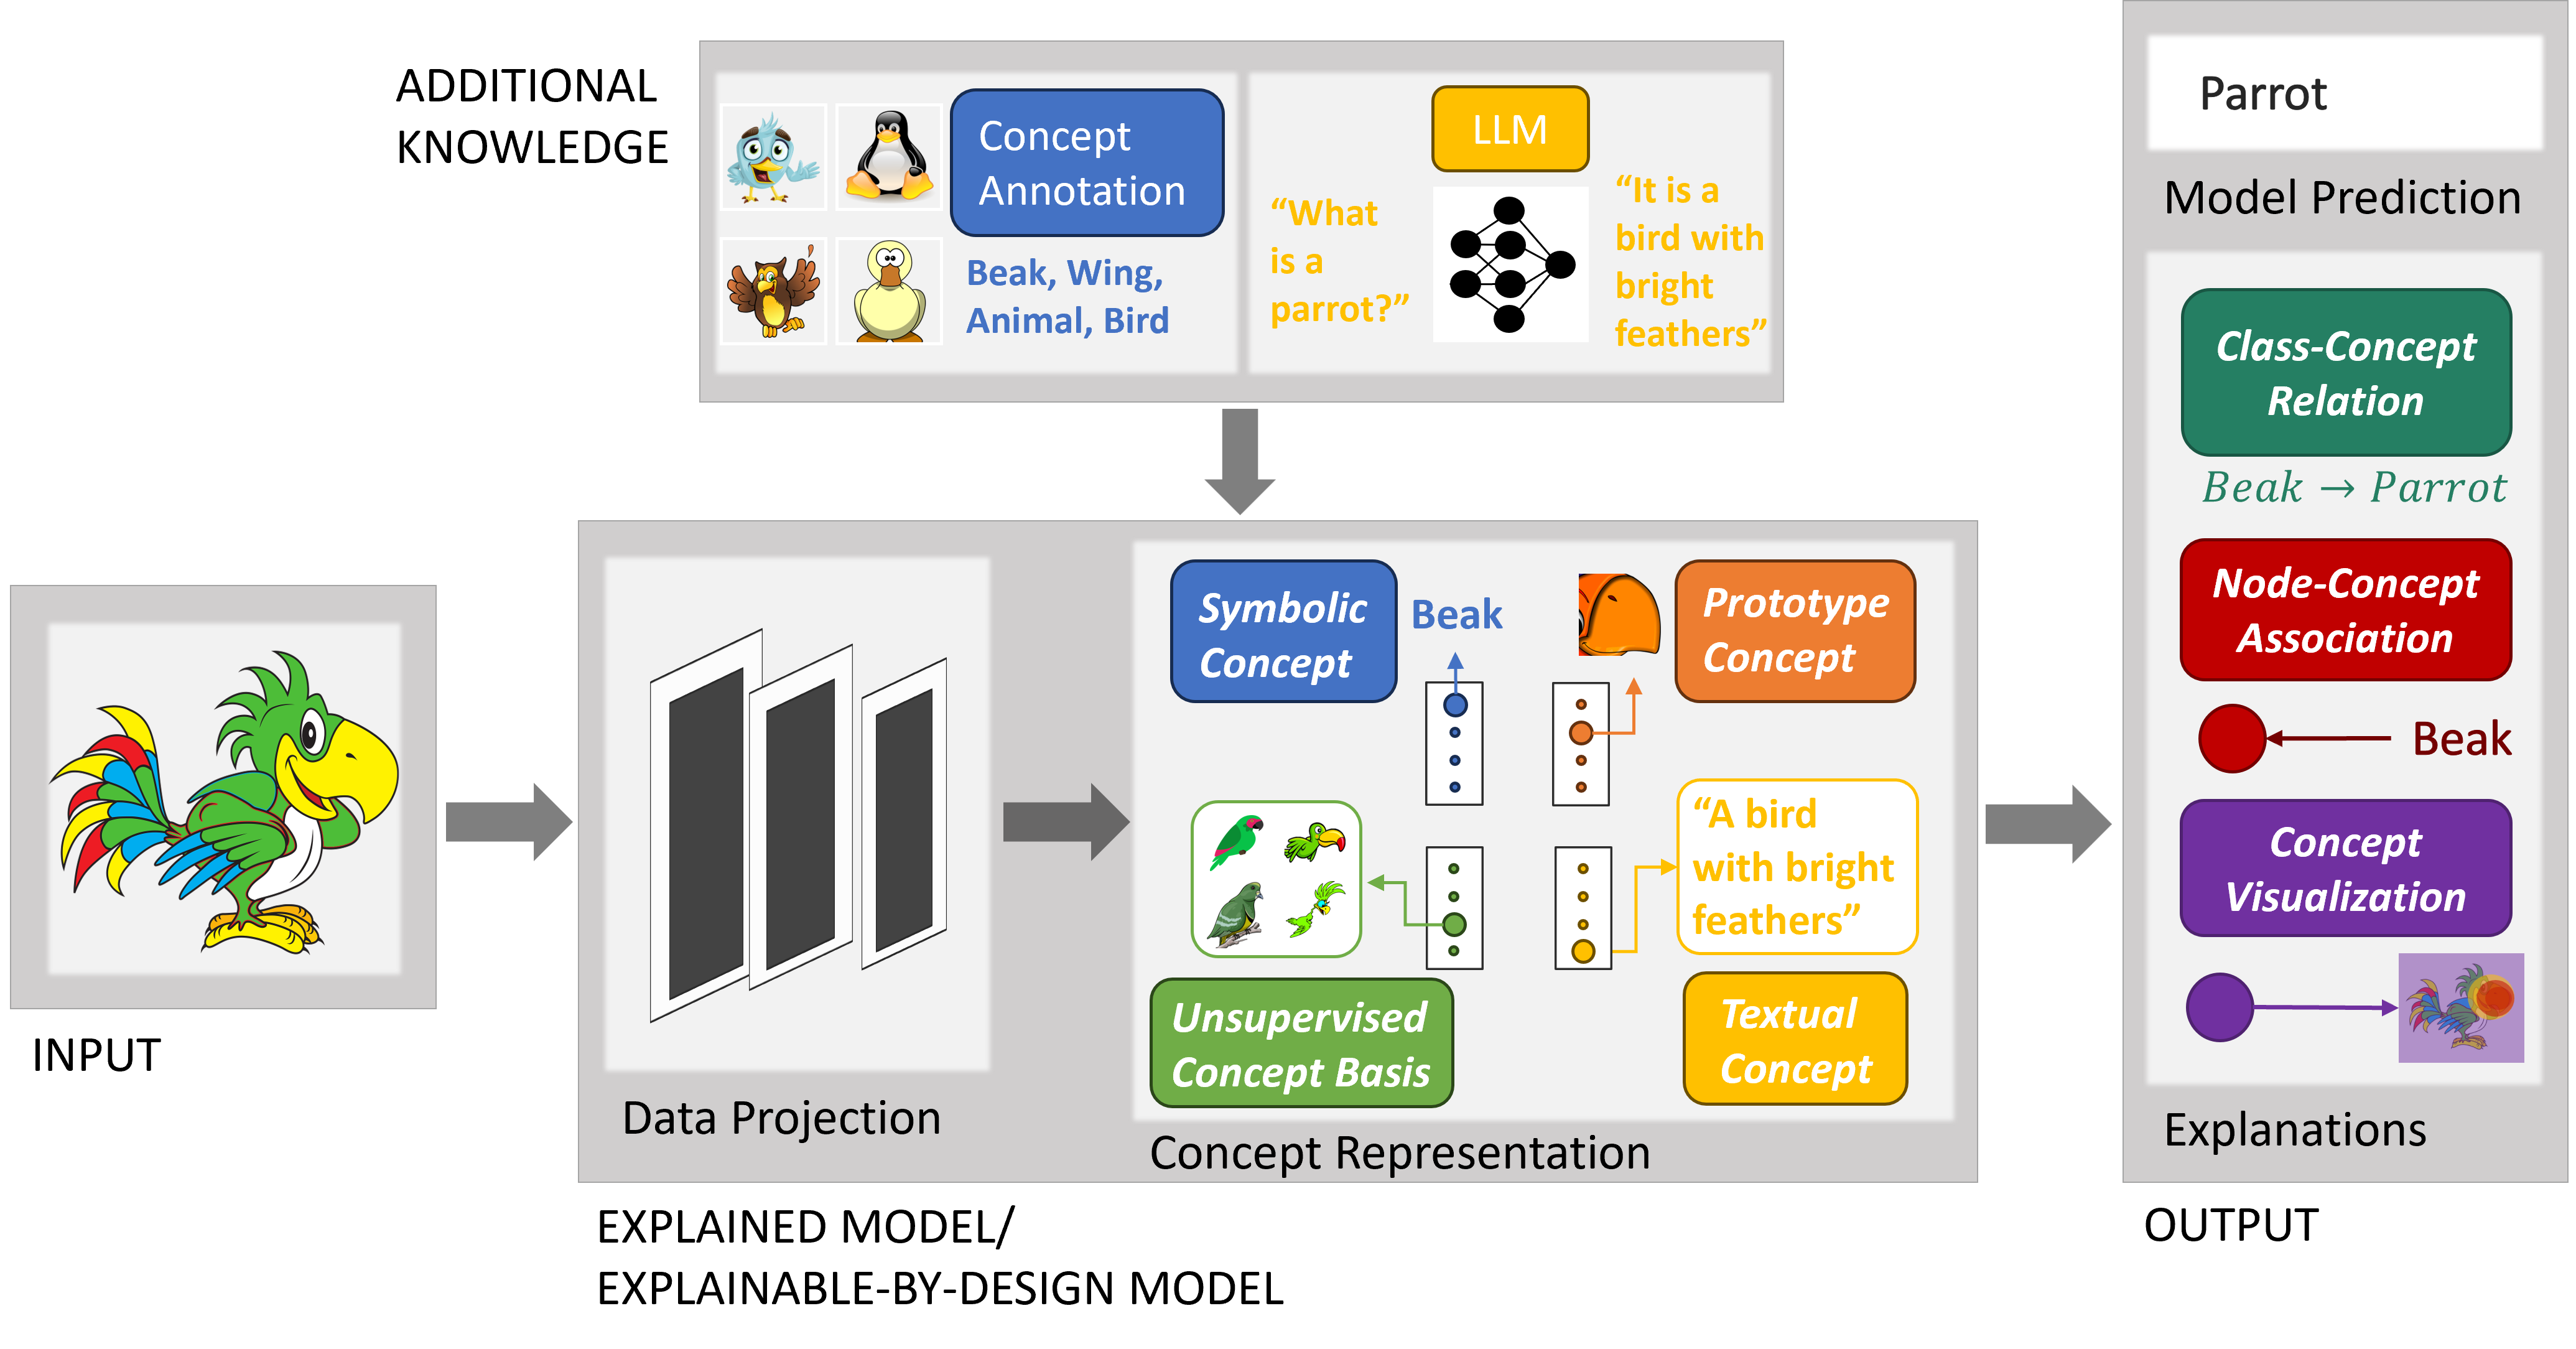
\includegraphics[width=0.9\textwidth]{images/C-XAI_defs_parrot.png}
        \caption{Types de concepts et d'explications à base de concepts \cite{poeta_concept-based_2023}}
        \label{fig:CXIA}
    \end{figure}
\end{frame}

\end{document}